\documentclass[a4paper,11pt]{article}
\usepackage[left=2.5cm,right=2.5cm,top=2.5cm]{geometry}
\usepackage[czech,slovak,english]{babel}
\usepackage[utf8]{inputenc}
\usepackage{url}
\usepackage{graphicx}
\usepackage{picture}
\usepackage{courier}
\usepackage{listings}

\addto\captionsenglish{\renewcommand{\figurename}{Obr.}}

\begin{document}

\section{Mesh Multiplication}
Mesh Multiplication je algoritmus pre výpočet násobku dvoch matíc. Obecne algoritmy pre výpočet násobku dvoch matíc očakávajú na vstupe dve matice A a B o rozmeroch $N \times M $ a $ M \times K $. Preto je základom algoritmu mriežka $N \times K $ procesorov. Každý procesor $ P(i, j) $ obsahuje register $ c_{i,j} $ obsahujúci hodnotu na i-tom riadku a j-tom stĺpci výslednej matice C.

Prvky matíc sa privádzajú do procesoru $ P(1,1)$. Prvky matice A sa privádzajú zľava a prvky matice B sa privádzajú zhora. S tým, že prvky nasledujúceho riadka alebo stĺpca sú o jednu pozíciu posunuté. Teda v prvom kroku sa vynásobia prvky $ a_{1,1} $ a $ b_{1,1} $, v ďalšom kroku sa prvok $ a_{1,1} $ posunie do procesoru $ P(1,2)$, kde sa vynásobí s prvkom $ b_{1,2} $, a podobne pokračuje ďalej. Obdobne algoritmus funguje aj pre prvky $b$. Algoritmus končí až sa vynásobia prvky $ a_{n,m} $ a $ b_{m,k} $.

\begin{figure}[!htb]
\centering
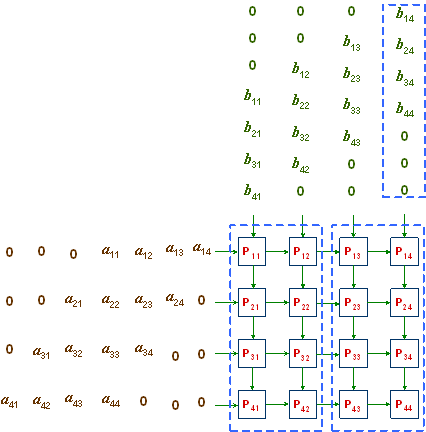
\includegraphics[width=60mm, scale=0.5]{mm.png}
\caption{Mesh Multiplication \fontsize{8pt}{12pt}\selectfont(Zdroj: https://web.njit.edu/~gilhc/labman/ECE459/e2.htm)}
\end{figure}

\subsection{Zložitosť}
Presná optimálna zložitosť algoritmu násobenia matíc nie je známa, ale je približne $O(n^x)$, kde $2<x<3$. Žiaden algoritmus nemá lepšiu zložitosť ako $O(n^2)$.
Prvky $ a_{n,1} $ a $ b_{1,k} $ potrebujú $m+k+n-2$ krokov, aby sa dostali k poslednému procesoru, preto:
\begin{itemize}
\item $ p(n,k) = n \cdot k = O(n^2)$
\item $ t(n) = m+n+k-2 = O(n) $
\item $ c(n) = t(n) \cdot p(n) = O(n)\cdot O(n^2) = O(n^3) $, čo nie je optimálna cena
\end{itemize}

\section{Vlastná implementácia algoritmu}
Výsledná implementácia sa od uvedeného algoritmu mierne líši. Hlavnou zmenou oproti vyššie popísanému algoritmu je, že hodnoty matíc A a B neprichádzajú pre nasledujúce riadky alebo stĺpce oneskorené, ale sú naraz poslané príslušnému procesoru. Akonáhle procesor obdrží hodnoty $ a_{i,m} $ a $ b_{m,k} $ vypočíta ich súčin, ten pripočíta k aktuálnej hodnote svojho registru C a hodnoty pošle susedným procesorom. Hodnotu $a$ procesoru $ P(i, j+1) $ ak $j<k$, a hodnotu $b$ procesoru $ P(i+1, j) $ ak $i<n$.

Komunikácia procesorov je znázornená na nasledovnom sekvenčnom diagrame. Zasielané správy v sekvenčnom diagrame majú formát $ v_{i,j} $, kde $v \in \{a, b, c\}$ je hodnota matice A, B alebo C (výsledná matica násobenia) v i-tom riadku a j-tom stĺpci.

\begin{figure}[!htb]
\centering
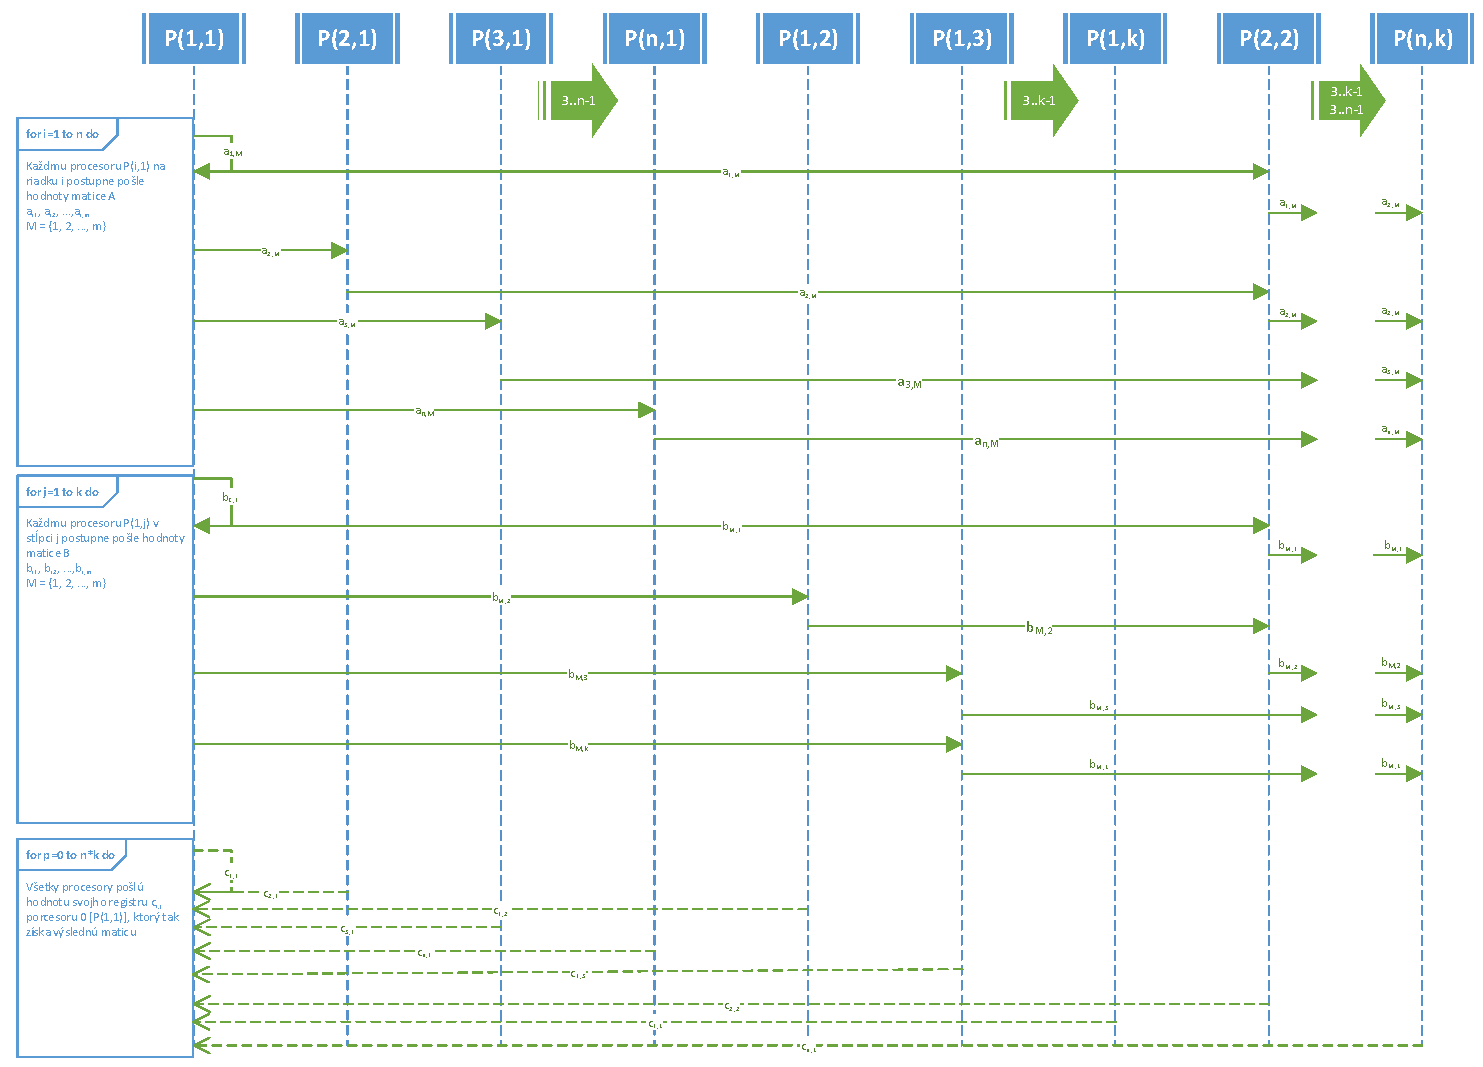
\includegraphics[width=\textwidth]{sequence.pdf}
\caption{Sekvenčný diagram}
\end{figure}

\subsection{Namerané hodnoty}
Na meranie času bola použitá funkcia \texttt{std::chrono::high\_resolution\_clock::now()} zo štandardnej knižnice C++ \texttt{chrono}. Meranie pre každú veľkosť vstupných dát bolo vykonané 10x na rovnakých maticiach. Násobené boli štvorcové matice rovnakých rozmerov ako výsledná matica. Namerané priemerné hodnoty pre rôzne veľkosti vstupu sú zobrazené v grafe na obrázku~\ref{stats}.

\begin{figure}[!htb]
\centering
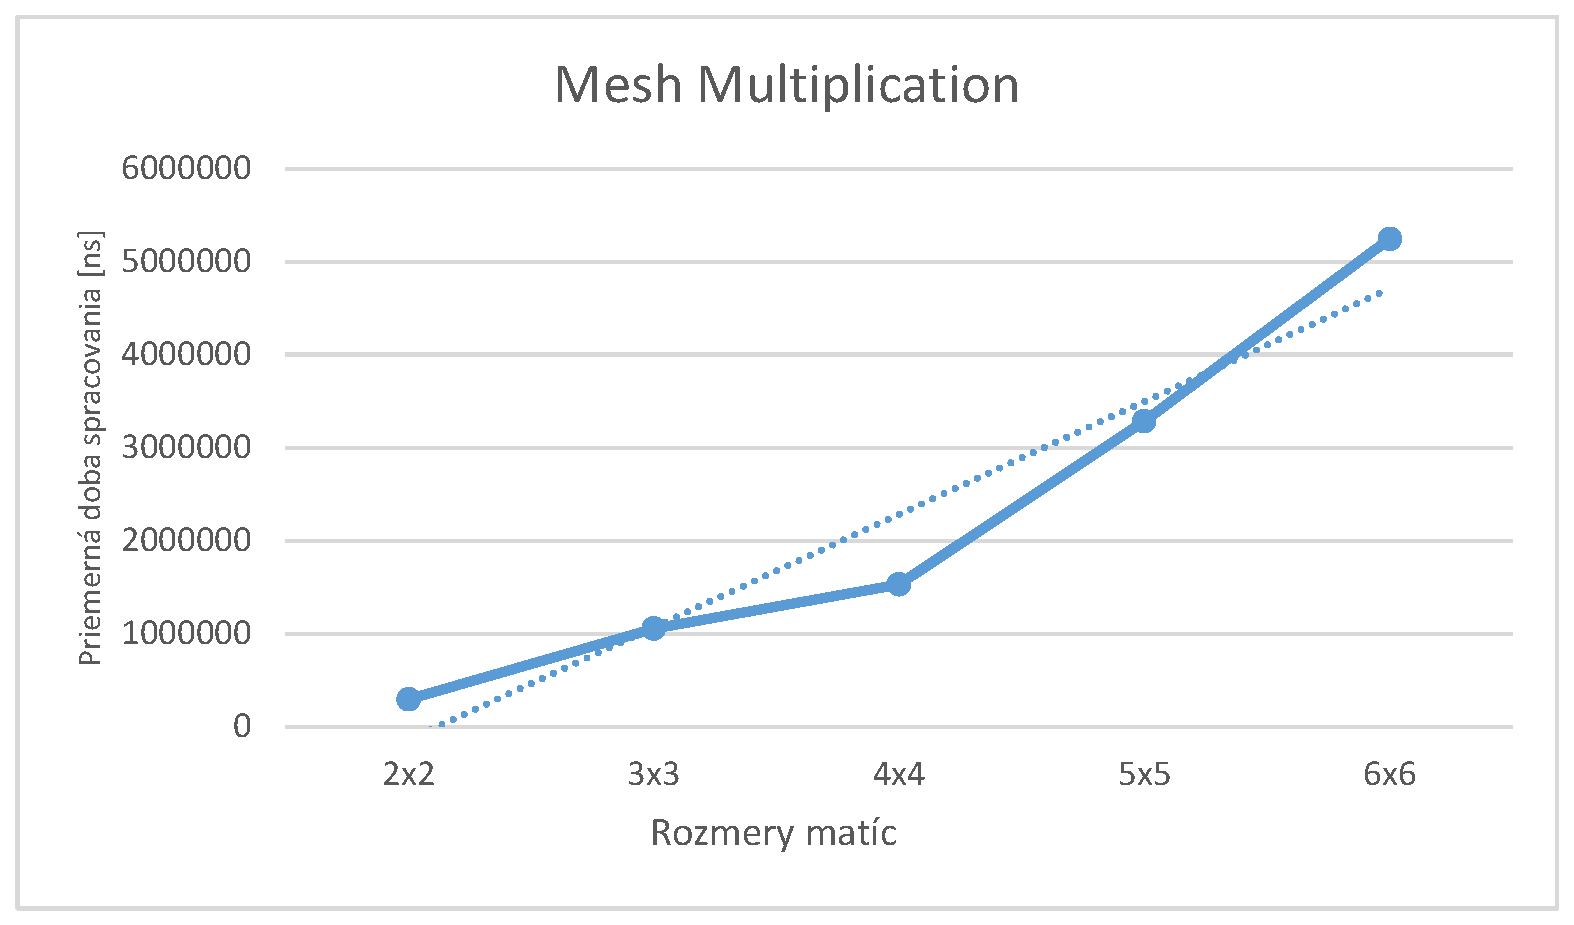
\includegraphics[width=\textwidth]{stats.pdf}
\caption{Namerané časy}
\label{stats}
\end{figure}

\makeatletter
\setlength{\@fptop}{0pt}
\makeatother

\section{Záver}
Z nameraných hodnôt znázornených v grafe možno vyvodiť, že implementovaný algoritmus dodržuje teoretickú lineárnu zložitosť algoritmu. Krivka s menšími odchýlkami kopíruje trendovú úsečku. Odchýlky sú spôsobené rozdielmi medzi jednotlivými meraniami, pretože pri niektorých meraniach došlo k 2-3 násobnému spomaleniu oproti ostatným pokusom. Zvýšením počtu meraní by sa dosiahli presnejšie výsledky.
\end{document}
